% Options for packages loaded elsewhere
\PassOptionsToPackage{unicode}{hyperref}
\PassOptionsToPackage{hyphens}{url}
%
\documentclass[
]{article}
\usepackage{lmodern}
\usepackage{amsmath}
\usepackage{ifxetex,ifluatex}
\ifnum 0\ifxetex 1\fi\ifluatex 1\fi=0 % if pdftex
  \usepackage[T1]{fontenc}
  \usepackage[utf8]{inputenc}
  \usepackage{textcomp} % provide euro and other symbols
  \usepackage{amssymb}
\else % if luatex or xetex
  \usepackage{unicode-math}
  \defaultfontfeatures{Scale=MatchLowercase}
  \defaultfontfeatures[\rmfamily]{Ligatures=TeX,Scale=1}
\fi
% Use upquote if available, for straight quotes in verbatim environments
\IfFileExists{upquote.sty}{\usepackage{upquote}}{}
\IfFileExists{microtype.sty}{% use microtype if available
  \usepackage[]{microtype}
  \UseMicrotypeSet[protrusion]{basicmath} % disable protrusion for tt fonts
}{}
\makeatletter
\@ifundefined{KOMAClassName}{% if non-KOMA class
  \IfFileExists{parskip.sty}{%
    \usepackage{parskip}
  }{% else
    \setlength{\parindent}{0pt}
    \setlength{\parskip}{6pt plus 2pt minus 1pt}}
}{% if KOMA class
  \KOMAoptions{parskip=half}}
\makeatother
\usepackage{xcolor}
\IfFileExists{xurl.sty}{\usepackage{xurl}}{} % add URL line breaks if available
\IfFileExists{bookmark.sty}{\usepackage{bookmark}}{\usepackage{hyperref}}
\hypersetup{
  hidelinks,
  pdfcreator={LaTeX via pandoc}}
\urlstyle{same} % disable monospaced font for URLs
\usepackage[margin=1in]{geometry}
\usepackage{graphicx}
\makeatletter
\def\maxwidth{\ifdim\Gin@nat@width>\linewidth\linewidth\else\Gin@nat@width\fi}
\def\maxheight{\ifdim\Gin@nat@height>\textheight\textheight\else\Gin@nat@height\fi}
\makeatother
% Scale images if necessary, so that they will not overflow the page
% margins by default, and it is still possible to overwrite the defaults
% using explicit options in \includegraphics[width, height, ...]{}
\setkeys{Gin}{width=\maxwidth,height=\maxheight,keepaspectratio}
% Set default figure placement to htbp
\makeatletter
\def\fps@figure{htbp}
\makeatother
\setlength{\emergencystretch}{3em} % prevent overfull lines
\providecommand{\tightlist}{%
  \setlength{\itemsep}{0pt}\setlength{\parskip}{0pt}}
\setcounter{secnumdepth}{-\maxdimen} % remove section numbering
\usepackage{booktabs}
\usepackage{longtable}
\usepackage{array}
\usepackage{multirow}
\usepackage{wrapfig}
\usepackage{float}
\usepackage{colortbl}
\usepackage{pdflscape}
\usepackage{tabu}
\usepackage{threeparttable}
\usepackage{threeparttablex}
\usepackage[normalem]{ulem}
\usepackage{makecell}
\usepackage{xcolor}
\ifluatex
  \usepackage{selnolig}  % disable illegal ligatures
\fi

\author{}
\date{\vspace{-2.5em}}

\begin{document}

\hypertarget{methods}{%
\section{Methods}\label{methods}}

The data collecting was done in a previous semester report, ``Is it
possible to predict movements in handball with machine learning using a
single inerntial measurement unit?'' (Lentz-Nielsen et al.~2021), which
was also conducted by the author of this report.

\vspace{0.5cm}

\hypertarget{participants}{%
\subsection{Participants}\label{participants}}

Five males and seven females participated in the study (\(21 \pm 2\)
years old, \(179 \pm 7\) cm, \(78 \pm 9\) kg, \(7 \pm 4\) years of
handball experience). They all had a high level of experience in
physical activities. Though, they had varying levels of experience with
handball ranging from beginners to former youth elite level players.
Subjects were informed of the structure of the test protocol, and signed
an informed consent prior to testing.

\begin{verbatim}
## -- Attaching packages --------------------------------------- tidyverse 1.3.1 --
\end{verbatim}

\begin{verbatim}
## v ggplot2 3.3.5     v purrr   0.3.4
## v tibble  3.1.4     v dplyr   1.0.7
## v tidyr   1.1.4     v stringr 1.4.0
## v readr   2.0.1     v forcats 0.5.1
\end{verbatim}

\begin{verbatim}
## -- Conflicts ------------------------------------------ tidyverse_conflicts() --
## x dplyr::filter() masks stats::filter()
## x dplyr::lag()    masks stats::lag()
\end{verbatim}

\begin{verbatim}
## 
## Vedhæfter pakke: 'kableExtra'
\end{verbatim}

\begin{verbatim}
## Det følgende objekt er maskeret fra 'package:dplyr':
## 
##     group_rows
\end{verbatim}

\begin{table}[H]

\caption{\label{tab:subjectInfo}Subject Information}
\centering
\begin{tabular}[t]{l|l|l|l|l|l|l|l}
\hline
\textbf{Subject} & \textbf{Sex} & \textbf{Team} & \textbf{Role} & \textbf{Age (yr)} & \textbf{Height (cm)} & \textbf{Weight (kg)} & \textbf{Experience (yr)}\\
\hline
\cellcolor{gray!6}{02} & \cellcolor{gray!6}{Male} & \cellcolor{gray!6}{B} & \cellcolor{gray!6}{Right} & \cellcolor{gray!6}{22} & \cellcolor{gray!6}{181} & \cellcolor{gray!6}{95} & \cellcolor{gray!6}{8}\\
\hline
04 & Female & A & Far left & 21 & 178 & 68 & 7\\
\hline
\cellcolor{gray!6}{05} & \cellcolor{gray!6}{Female} & \cellcolor{gray!6}{B} & \cellcolor{gray!6}{Left} & \cellcolor{gray!6}{23} & \cellcolor{gray!6}{164} & \cellcolor{gray!6}{72} & \cellcolor{gray!6}{1}\\
\hline
06 & Female & B & Far Left & 20 & 171 & 70 & 7\\
\hline
\cellcolor{gray!6}{07} & \cellcolor{gray!6}{Female} & \cellcolor{gray!6}{A} & \cellcolor{gray!6}{Right} & \cellcolor{gray!6}{22} & \cellcolor{gray!6}{179} & \cellcolor{gray!6}{72} & \cellcolor{gray!6}{10}\\
\hline
08 & Male & A & Line & 21 & 193 & 85 & 1\\
\hline
\cellcolor{gray!6}{09} & \cellcolor{gray!6}{Female} & \cellcolor{gray!6}{A} & \cellcolor{gray!6}{Far right} & \cellcolor{gray!6}{20} & \cellcolor{gray!6}{175} & \cellcolor{gray!6}{76} & \cellcolor{gray!6}{5}\\
\hline
10 & Male & A & Playmaker & 20 & 178 & 84 & 7\\
\hline
\cellcolor{gray!6}{11} & \cellcolor{gray!6}{Male} & \cellcolor{gray!6}{A} & \cellcolor{gray!6}{Left} & \cellcolor{gray!6}{26} & \cellcolor{gray!6}{186} & \cellcolor{gray!6}{85} & \cellcolor{gray!6}{9}\\
\hline
15 & Male & B & Playmaker & 21 & 186 & 90 & 17\\
\hline
\cellcolor{gray!6}{16} & \cellcolor{gray!6}{Female} & \cellcolor{gray!6}{B} & \cellcolor{gray!6}{Line} & \cellcolor{gray!6}{22} & \cellcolor{gray!6}{183} & \cellcolor{gray!6}{78} & \cellcolor{gray!6}{5}\\
\hline
17 & Female & B & Far right & 19 & 175 & 64 & 3\\
\hline
\hline
\cellcolor{gray!6}{$Average \pm sd$} & \cellcolor{gray!6}{} & \cellcolor{gray!6}{} & \cellcolor{gray!6}{} & \cellcolor{gray!6}{$21 \pm 2$} & \cellcolor{gray!6}{$179 \pm 7$} & \cellcolor{gray!6}{$78 \pm 9$} & \cellcolor{gray!6}{$7 \pm 4$}\\
\hline
\end{tabular}
\end{table}

\hypertarget{protocol-design}{%
\subsection{Protocol design}\label{protocol-design}}

\hypertarget{technical-design}{%
\subsubsection{Technical design}\label{technical-design}}

In this cross-sectional study, 3D acceleration and 3D rotation was
measured with an IMU to develop a supervised machine learning algorithm
to detect handball events within a regular handball match (introduced in
section @ref(labeling)). Video recordings were collected and used to
label each event as the ground-truth for the supervised machine learning
algorithm to train and test on. To measure the inertial sensor data,
players wore a vest with a Catapult Vector S7 placed between the
scapulae on the upper back. Triaxial accelerometers and the gyroscope
had a range of \(3D \pm 16g\), and \(2000^{\circ}/s\) respectively,
which collected data, at 100Hz. A magnetometer was also part of the IMU
(see figure @ref(fig:globalSystem)).

\begin{figure}
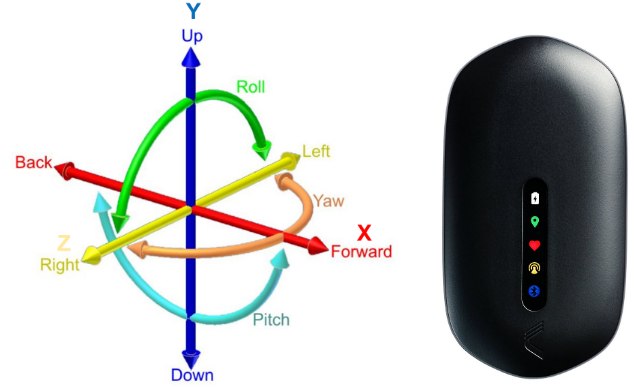
\includegraphics[width=1\linewidth]{img/globalSystem} \caption{Orientation of the IMU sensor}\label{fig:globalSystem}
\end{figure}

Videos were recorded by two GoPro Hero 7 cameras at 48fps and a
resolution of 1920x1080 pixels. The cameras were placed approximately 5
m behind each bacline and 3 m above the playing field, with an angle at
roughly \(15^{\circ}\) relative to the ground, to make a whole field
recording possible.

To ensure synchronization between the IMUs and cameras, four
interrupting periods were implemented to the handball match. One in the
beginning and three during the match with 5 min in between. During the
interruptions the players were instructed to stop all movement for 10 s,
then do three jumps with 1 s in between and subsequently stand still for
10 s before returning to the match. These periods were easily detectable
on IMU recordings. The pauses were controlled by the handball referee.

To ensure correct mapping of the devices to the subjects, a manual
exploration of the raw data was conducted. The pattern from the yaw
velocity during hard overhead throws was easily detectable in the data
and ensured correct mapping (see figure @ref(fig:yawPhoto)).

\begin{figure}
\includegraphics[width=1\linewidth]{img/yawPhoto} \caption{Graph represents one of the subjects performing a hard overhead throw. With yaw velocity on the y axis and time on the x axis. The pictures is the physical movements the graph is recorded from. }\label{fig:yawPhoto}
\end{figure}

\hypertarget{practical-design}{%
\subsubsection{Practical design}\label{practical-design}}

Prior to the match all players participated in a self-paced warm up
routine that had a primary focus to warm up the ankle-. knee-, and
shoulder joints. Two matches of 20 min. duration were arranged. Six
field players were on each team (Team A and Team B). A limited number of
IMUs were available to monitor all players simultaneously, therefore two
matches were held. Team A was recorded in the first match and team B in
the second. None of the teams were allowed any substitutions and a 15
min. break separated the two matches where the equipment was cleaned and
placed on the second team.

\hypertarget{labeling}{%
\subsection{Labeling}\label{labeling}}

The specific events in handball relevant for the current study to
research, were selected based on the physical demands of the sport.
These demands can be classified as either locomotion, e.g., walking and
running, or technical events e.g.~throws \citep{Michalsik2018}. To
facilitate the classification, the use of IMUs were chosen in addition
to video recordings. The video recordings were used as the ground truth
for each performed event. Consequently, three events was chosen to
describe the locomotion movements; Low Intensity (LI), Running, and
Dynamic. Overhead throws was chosen as the only technical throw event to
label. This was to ensure that the IMU could detect the throws
\citep{Skejo2021}.

\begin{table}[H]

\caption{\label{tab:labels}Labels and their descriptions}
\centering
\begin{tabular}[t]{l|l}
\hline
\textbf{Labels} & \textbf{Description}\\
\hline
\cellcolor{gray!6}{Low Intensity} & \cellcolor{gray!6}{Standing and walking like movements}\\
\hline
Running & Steady state linear and curved jogging and running\\
\hline
\cellcolor{gray!6}{Dynamic} & \cellcolor{gray!6}{Multi directional movements}\\
\hline
Throw & Only overhead throws\\
\hline
\end{tabular}
\end{table}

The labeling process was done with Catapult Vision v5.2.0 software,
where each locomotion event was manually labeled with a dynamic length
for each occurence of the event. The overhead throws is an instantaneous
event therefore the labeling of these was done with 0.5s before and
after the release of the ball which results in a one second static
length of each overhead throw occurence.

\hypertarget{data-processing}{%
\subsection{Data processing}\label{data-processing}}

The changes in the orientation of the IMU sensor was accounted for by a
Kalman Filter provided by the manufacturer (KILDE). The algorithm
accuracy has been validated for sports specific use
\citep{Wundersitz2013, Wundersitz2015}. Hereafter the inertial data and
labeling data was imported to R statistical software package v4.1.1,
where the synchronized labels were applied to the synchronized IMU data
in respect to the subject and time. Each occurence of the events listed
in table @ref(tab:labels) was enumerated by a unique occurence ID; the
first time Dynamic movement occurs for subject one, it will recieve the
occurence ID \#1. The second time it occurs, it will get the occurence
ID \#2 and so on.

Prior to the feature engineering a lowpass zero-phase 2nd order 5 Hz
Butterworth filter was implemented, to attenuate frequencies above the
chosen cut-off. A visual representation of the filter was created (see
figure @ref(fig:lowpassFilter)) to verify the chosen filter. Where plot
A and B shows the forward acceleration in the time domain prior and
after the implementation of the filter, respectively. Plot C and D shows
the same acceleration vector but in the frequency domain before and
after the implementation of the filter, respectively.

\begin{figure}
\includegraphics[width=1\linewidth]{img/signalfilter} \caption{Forward acceleration showed in time (A,B) and frequency (C,D) domain. The left plots (A,C) is before filtering and the right plots (B,D) is after filtering.}\label{fig:lowpassFilter}
\end{figure}

Furthermore, the linear trend from each acceleration axis was applied to
remove a possible bias and drift in the data. This also removes the
gravitation component from the output of the accelerometers.

\hypertarget{feature-engineering}{%
\subsection{Feature engineering}\label{feature-engineering}}

An overview of the workflow from the processed data to validating the
model can be see in figure @ref(fig:featureWorkflow)

\begin{figure}
\includegraphics[width=1\linewidth]{img/featureworkflow1} \caption{Showing the workflow from time series to validation of the model}\label{fig:featureWorkflow}
\end{figure}

First a few new time series features was created; Acceleration
magnitude, angular magnitude and triaxial velcoities. From here 7
aggregated features was calculated with the use of a one second rolling
window with no overlap on each time series; mean, median, max, min, 10th
percentile, 90th percentile and inter quartile range (IQR)

After calculation of the aggregated features a feature selection
approach was done executed. ``Variable Selection Using Random Forest''
(VSURF) \citep{Genuer2010, Genuer2015} package within R was used to
extract the most important variables and discard the once which would
not contribute to higher classification accuracy.

\hypertarget{training-the-models}{%
\subsection{Training the models}\label{training-the-models}}

The data was split into a training and test set by the
``leave-one-subject-out'' approach. A v-fold cross validation was used
on the training set to tune the hyperparameters for each model. Three
preprocessing approaches were used: No upsampling, SMOTE
\citep{Chawla2002} and ADASYN \citep{He2008}. These where then used in
four different models: Support Vector Machine with a radial basis
kernel, K-Nearest Neighbor, Random Forest and Extreme Gradient Boosted
Tree. All models was tuned for hyperparameters with the use of the
\emph{tune\_race\_anova} function from the \emph{finetune} v0.1.0
package in R. The best performing models was chosen based on the
F-measure and Matthews Correlation Coefficient (MCC). The F-measure
represents the harmonic mean of precision and recall. The F-measure is
chosen above accuracy because of the lack of an even distribution in the
labels, while also being a better metric when false negatives and false
positives are of importance \citep{Kelleher2015}. Together with the
F-measure the MCC was chosen \citep{Delgado2019}. MCC measures the
difference between actual and predicted value and also takes imbalanced
data into account as well.

This approach would be repeated for each subject in the data. The first
iteration would have Subject 02 pulled out and used as the test set, the
secon iteration would have Subject 04 pulled out and used as the test
set and so on.

\end{document}
